%%%%%%%%%%%%%%%%%%%%%%%%%%%%%%%%%%%%%%%%%%%%%%%%%%%%%%%%%%%%%%%%%%%%%%%%
%
%
%     This file is included from the file   Segmentation.tex
% 
%     Section tag and label are placed in this top file.
%
%
%
%%%%%%%%%%%%%%%%%%%%%%%%%%%%%%%%%%%%%%%%%%%%%%%%%%%%%%%%%%%%%%%%%%%%%%%%

\subsection{Introduction}
\label{sec:HybridSegmentationIntroduction}


Hybrid methods for automated segmentation of radiological patient data and the 
Visible Human data integrate boundary-based and region-based segmentation methods 
that amplify the strength but reduces the weakness of both approaches.The novelty 
comes from combining a region-based segmentation methods, the fuzzy connectedness 
and Voronoi Diagram classification with a boundary-based deformable model 
segmentation, to develop hybrid methods that yield high precision, accuracy and 
efficiency.The synergy between fundamentally different methodologies tends to 
result in robustness and higher segmentation quality. We built Hybrid Segmentation 
Engine,  Figure \ref{fig:ComponentsofaHybridSegmentationApproach}, that consists of modules 
representating component segmentation methods (itk filters). We can derive a variety 
of hybrid segmentation methods from the modules. It should be noted that under Fuzzy 
Connectedness module and Deformable Models module, we checked in into the itk a number 
of filters in each of the categories, respectively. Below, we decribe two examples of
hybrid segmentation methods, derived from the Hybrid segmentation Engine: Hybrid 
Method 1: Integration of Fuzzy Connectedness and Voronoi Diagram Classification;
Hybrid Method 2: Integration of Gibbs prior and Deformable Models.
Details on the concepts behind those methods have been discussed in the
literature
\cite{Angelini2002,Udupa2002,Jin2002,Imielinska2001,Imielinska2000a,Imielinska2000b}



\subsection{HybridMethod1:FuzzyConectednessAndVoronoiDiagramClassification}
\label{sec:HybridMethod1}

In this section, we present a hybrid segmentation method that requires minimal
manual initialization, where we integrate the fuzzy connectedness segmentation
and Voronoi Diagram Classification. We start with fuzzy connectedness filter
to generate a sample of tissue from a region to be segmented. From the sample,
we derive automatically, homogeneity statistics that constitute homogeneity
operator to be used in the next stage of the method. The output of the fuzzy 
connectedness filter is used as a prior for the Voronoi Diagram Classification 
filter that performs iterative subdivision and classification of the segmented
image that results in an estimation of the boundary. The output of this filter
is a 3D binary image that can be used to display the 3D result of the
segmentation, or passed to another filter (e.g. Deformable Model) for further
improvement of the final segmentation. Details describing the concepts behind those methods 
have been published in
\cite{Angelini2002,Udupa2002,Jin2002,Imielinska2001,Imielinska2000a,Imielinska2000b}

In Figure \ref{fig:UMLClassDiagramoftherFuzzyConnectednessFilter}, we describe 
base class for simple fuzzy connectedness segmentation. This method is non-scale 
based, non-iterative and requires only one seed to initialize it. We define affinity 
between two nearby elements in a image (e.g. pixels, voxels) via a degree of adjacency, 
similarity of their intensity values, and their similarity with the estimated object. 
The closer the elements are and more similar their intensities are, the greater is 
the affinity between them. We compute the strength of a path and fuzzy connectedness 
between each two pixels (voxels) in the segmented image from the fuzzy affinity. 
Computation of fuzzy connectedness value of each pixel (voxel) is implemented
by selecteing a seed point and using dynamic programming. The result constitutes the fuzzy
map. Thresholding of the fuzzy map gives a segmented object that is strongly connected
to the seed point (for more details, see \cite{Udupa1996}). We checked in two fuzzy 
connectedness filters: the itkSimpleFuzzyConnectednessScalarImageFilter that is an
implementation of the fuzzy connectedness segmentation of single channel (gray scale) 
image;itkSimpleFuzzyConnectednessRGBImageFilter that is an implementation of fuzzy
connectedness implementation of three-channel (RGB) image. Other classes can be derived 
from the base class by defining other affinity function, and targeting multi-channel
images with and arbitrary number of channels. It has to be noted, that the simple fuzzy 
connectedness filter can be used as a stand-alone segmentation method,
as it is described in the diagram in Figure 
\ref{fig:UMLCollaborationDiagramoftheFuzzyConnectednessFilter}.

In Figure \ref{UMLVoronoiSegmentationClassFilter} we present base class for Voronoi
Diagram Clasification. We initialize the method with a number of random seed points and compute
Voronoi Diagram over the segmented 2D image. Each Voronoi region, in teh subdivision,
is classified as internal
or external, based on the homogeneity operator derived from the fuzzy connectedness algorithm.
We define boundary regions as the external regions that are adjacent to the internal regions. 
We subdivide further the boundary regions by adding seed points to
the regions. We converge to the final segmentation using simple stopping criterium (for details,
see \cite{Imielinska2001}). We implemneted two Voronoi Diagram filters:
the itkVoronoiSegmentationImageFilter that is dedicated to process single
channel (gray scale) images; the itkVoronoiSegmentationRGBImageFilter that segments three-channel
(RGB) images. Other classes can be derivedfrom the base class by defining other homogeneity
measurements, and targeting multichannel images with and arbitrary number of channels.
The other classes that are used for computing 2D Voronoi Diagram, are shown in Figure \ref{fig:UMLClassesforImplementationofVoronoiDiagramFilter}}. We note that the Voronoi Diagram
Filter can be used as a stand-alone segmentation method, as it is depicted in Figure
\ref{fig:UMLCollaborationDiagramoftheVoronoiSegmentationFilter}.

 We present in Figure \ref{fig:UMLHybridMethodDiagram1} Figure \ref{fig:UMLHybridMethodDiagram2} d
diagrams for hybrid segmentation methods that integrate: fuzzy connectednedd with Voronoi Diagram;
and fuzzy connectedness, Voronoi Diagram with Deformable Models, respectively.


%%%%%%%%%%%%%%%%%%%%%%%%%%%%%%%%%%%%%%%%%%%%%%%%%%%%%%%%%%%%%%%%%
%
%  Here is an example of how to include diagram in a figure
%
%  The file HybridSegmentationDiagram1.fig should be in the "Art"
%  directory. CMake will convert it to EPS before running latex. 
%
%%%%%%%%%%%%%%%%%%%%%%%%%%%%%%%%%%%%%%%%%%%%%%%%%%%%%%%%%%%%%%%%%

\begin{figure}
\center
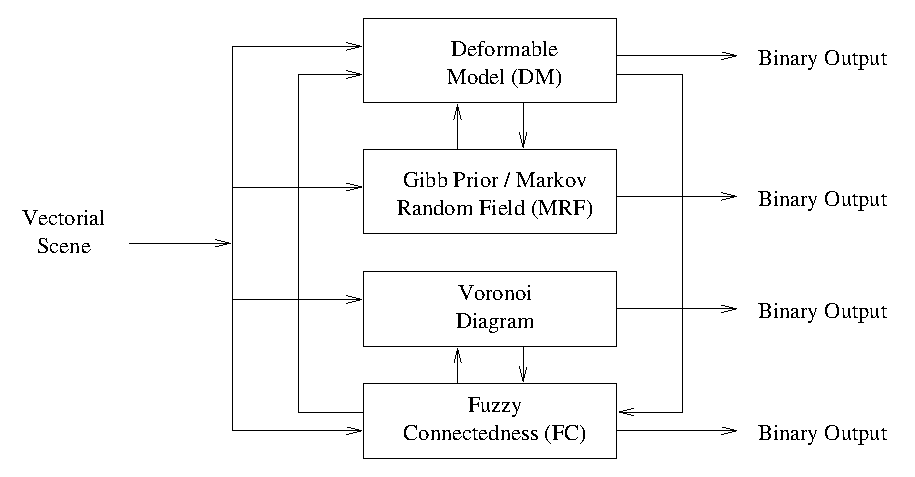
\includegraphics[width=14cm]{HybridSegmentationEngine1.eps}
\caption{Hybrid Segmentation Engine}
\label{fig:ComponentsofaHybridSegmentationApproach}
\end{figure}


\begin{figure}
\center
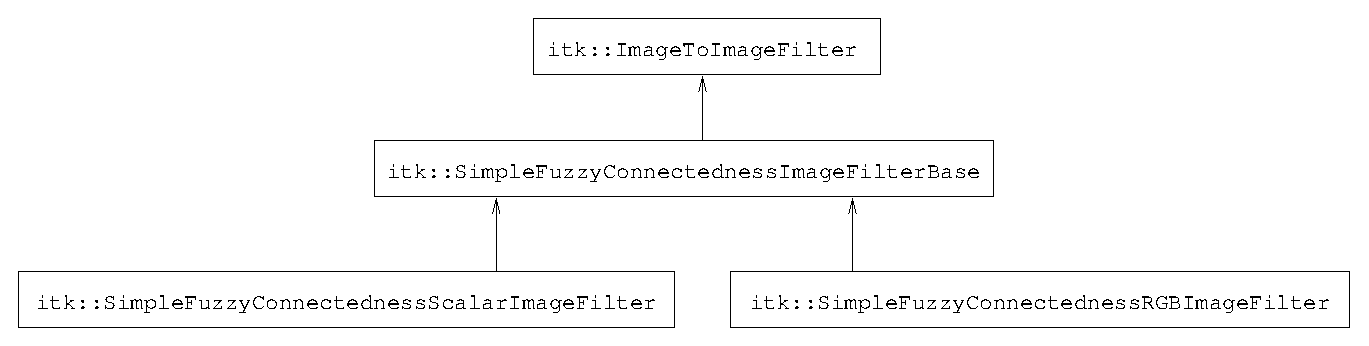
\includegraphics[width=14cm]{FuzzyConnectednessClassDiagram1.eps}
\caption{Diagram of the FuzzyConnectedness filter}
\label{fig:UMLClassDiagramoftherFuzzyConnectednessFilter}
\end{figure}


\begin{figure}
\center
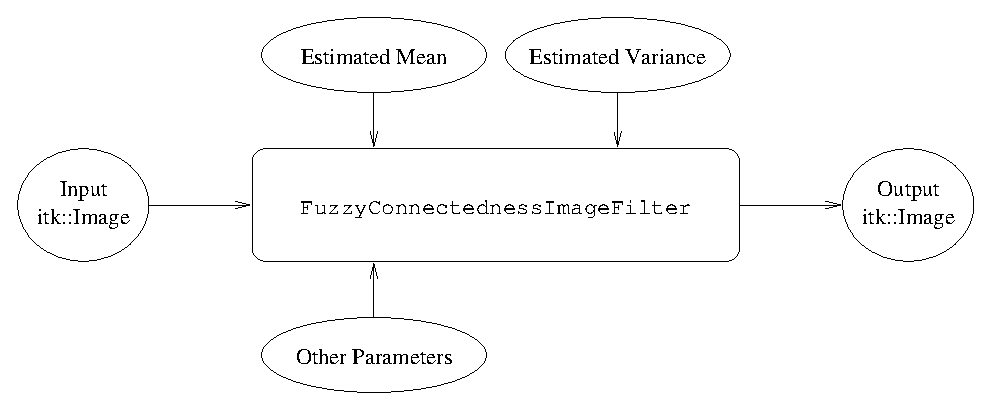
\includegraphics[width=14cm]{FuzzyConnectednessCollaborationDiagram1.eps}
\caption{Diagram Of Stand-Alone Fuzzy Connectedness Segmentation}
\label{fig:UMLCollaborationDiagramoftherFuzzyConnectednessFilter}
\end{figure}

\begin{figure}
\center
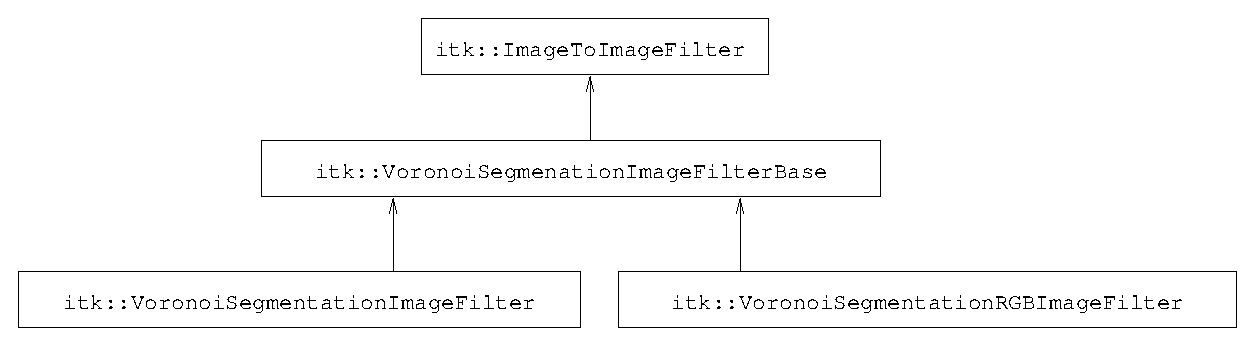
\includegraphics[width=14cm]{VoronoiSegmentationClassDiagram1.eps}
\caption{Diagram of the Voronoi Diagram Classification filter}
\label{fig:UMLVoronoiSegmentationClassFilter}
\end{figure}

\begin{figure}
\center
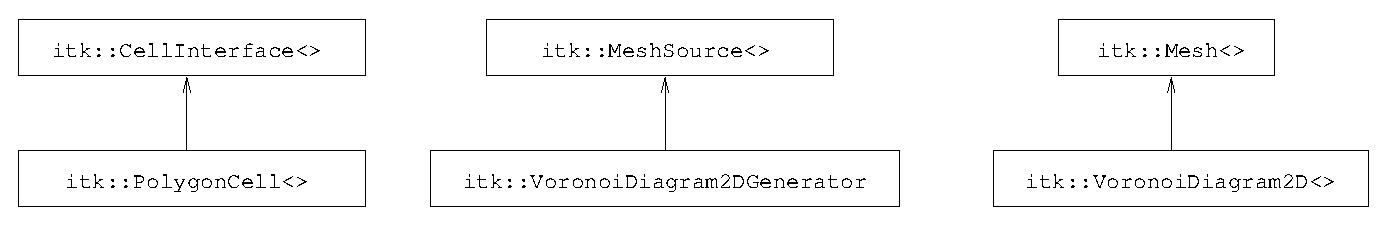
\includegraphics[width=14cm]{VoronoiSegmentationCollaborationDiagram1.eps}
\caption{Classes for Implementation of Voronoi Diagram Filter}
\label{fig:UMLClassesforImplementationofVoronoiDiagramFilter}
\end{figure}


\begin{figure}
\center
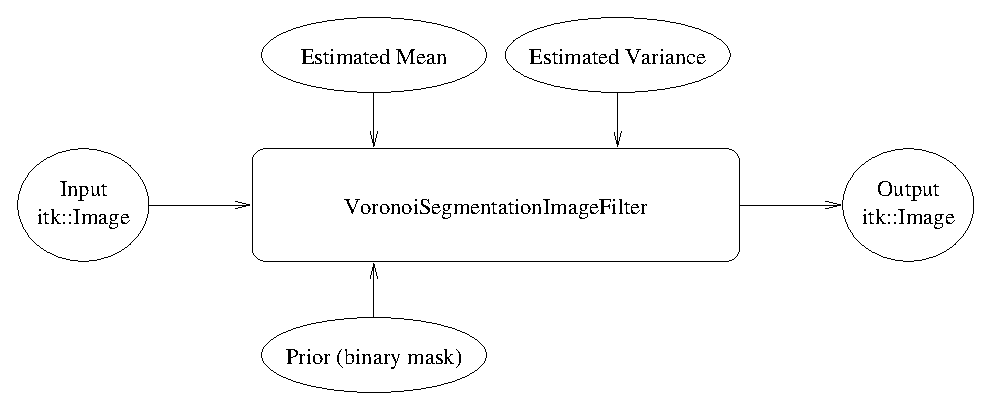
\includegraphics[width=14cm]{VoronoiSegmentationCollaborationDiagram2.eps}
\caption{Diagram Of Stand-Alone Voronoi Diagram Segmentation}
\label{fig:UMLCollaborationDiagramoftheVoronoiSegmentationFilter}
\end{figure}


\begin{figure}
\center
\includegraphics[width=14cm]{HybridMethodDiagram1.eps}
\caption{Integration of Fuzzy Connectedness with Voronoi Diagram Classification}
\label{fig:UMLHybridMethodDiagram1}
\end{figure}

\begin{figure}
\center
\includegraphics[width=14cm]{HybridMethodDiagram22.eps}
\caption{Integration of Fuzzy Connectedness, Voronoi Diagram, and Deformable Models}
\label{fig:UMLHybridMethodDiagram2}
\end{figure}



\subsubsection{HybridMethod1:Example}
\label{sec:HybridMethod1:Example}

The source code of this section can be found in the file 
Examples/Segmentation/HybridSegmentationFuzzyVoronoi.cxx

\input{HybridSegmentationFuzzyVoronoi.tex}


\subsection{HybridMethod2:GibbsPriorDeformableModel}
\label{sec:HybridMethod2}


\subsubsection{HybridMethod2:Example}
\label{sec:HybridMethod2:Example}

